\documentclass[a4paper]{article}
\usepackage[warn]{mathtext}
\usepackage[utf8]{inputenc}
\usepackage[T2A]{fontenc}
\usepackage[english,russian]{babel}
\usepackage{booktabs}
\usepackage{multicol}
\usepackage{fancyhdr}
\usepackage{graphicx}
\usepackage{microtype}
\usepackage{wrapfig}
\usepackage{amsmath}
\usepackage{floatflt}
\usepackage{geometry} \geometry{verbose,a4paper,tmargin=2cm,bmargin=2cm,lmargin=1.5cm,rmargin=1.5cm}
\usepackage{float}
\usepackage{amssymb}
\usepackage{caption}
\usepackage{epsfig}
\usepackage{newunicodechar}

\begin{document}

\graphicspath{ {pictures/} }
\begin{center}
    {\scshape\Large Лабораторная работа по квантовой электронике} \par

    \

    {\huge\bfseries № 26. Пространственные характеристики излучения ИПЛ} \par 

    \

    {\large Яромир Водзяновский Б04-855а}
\end{center}

\

\
\section{Введение}

\subsection{Цель работы} 
\begin{enumerate}
    \item Исследовать диаграммы направленности излучения полупроводникового инжекционного лазера в плоскости активного слоя и в плоскости, перпендикулярной активному слою.
\end{enumerate}

\subsection{Суть работы}

Используя вращающийся фотодетектор, который снимает зависимость интенсивности, пропорциональной получаемому в опыте напряжению, приходящего на него лазерного излучения от угла поворота. 
Возможно ограничить распространение сигнала с помощью щели, расположив её перпендикулярно активной среде.
    
\section{Эксперимент}

\subsection{Щель расположена перпендикулярно активному слою}

\begin{figure}[H]
    \begin{center}
        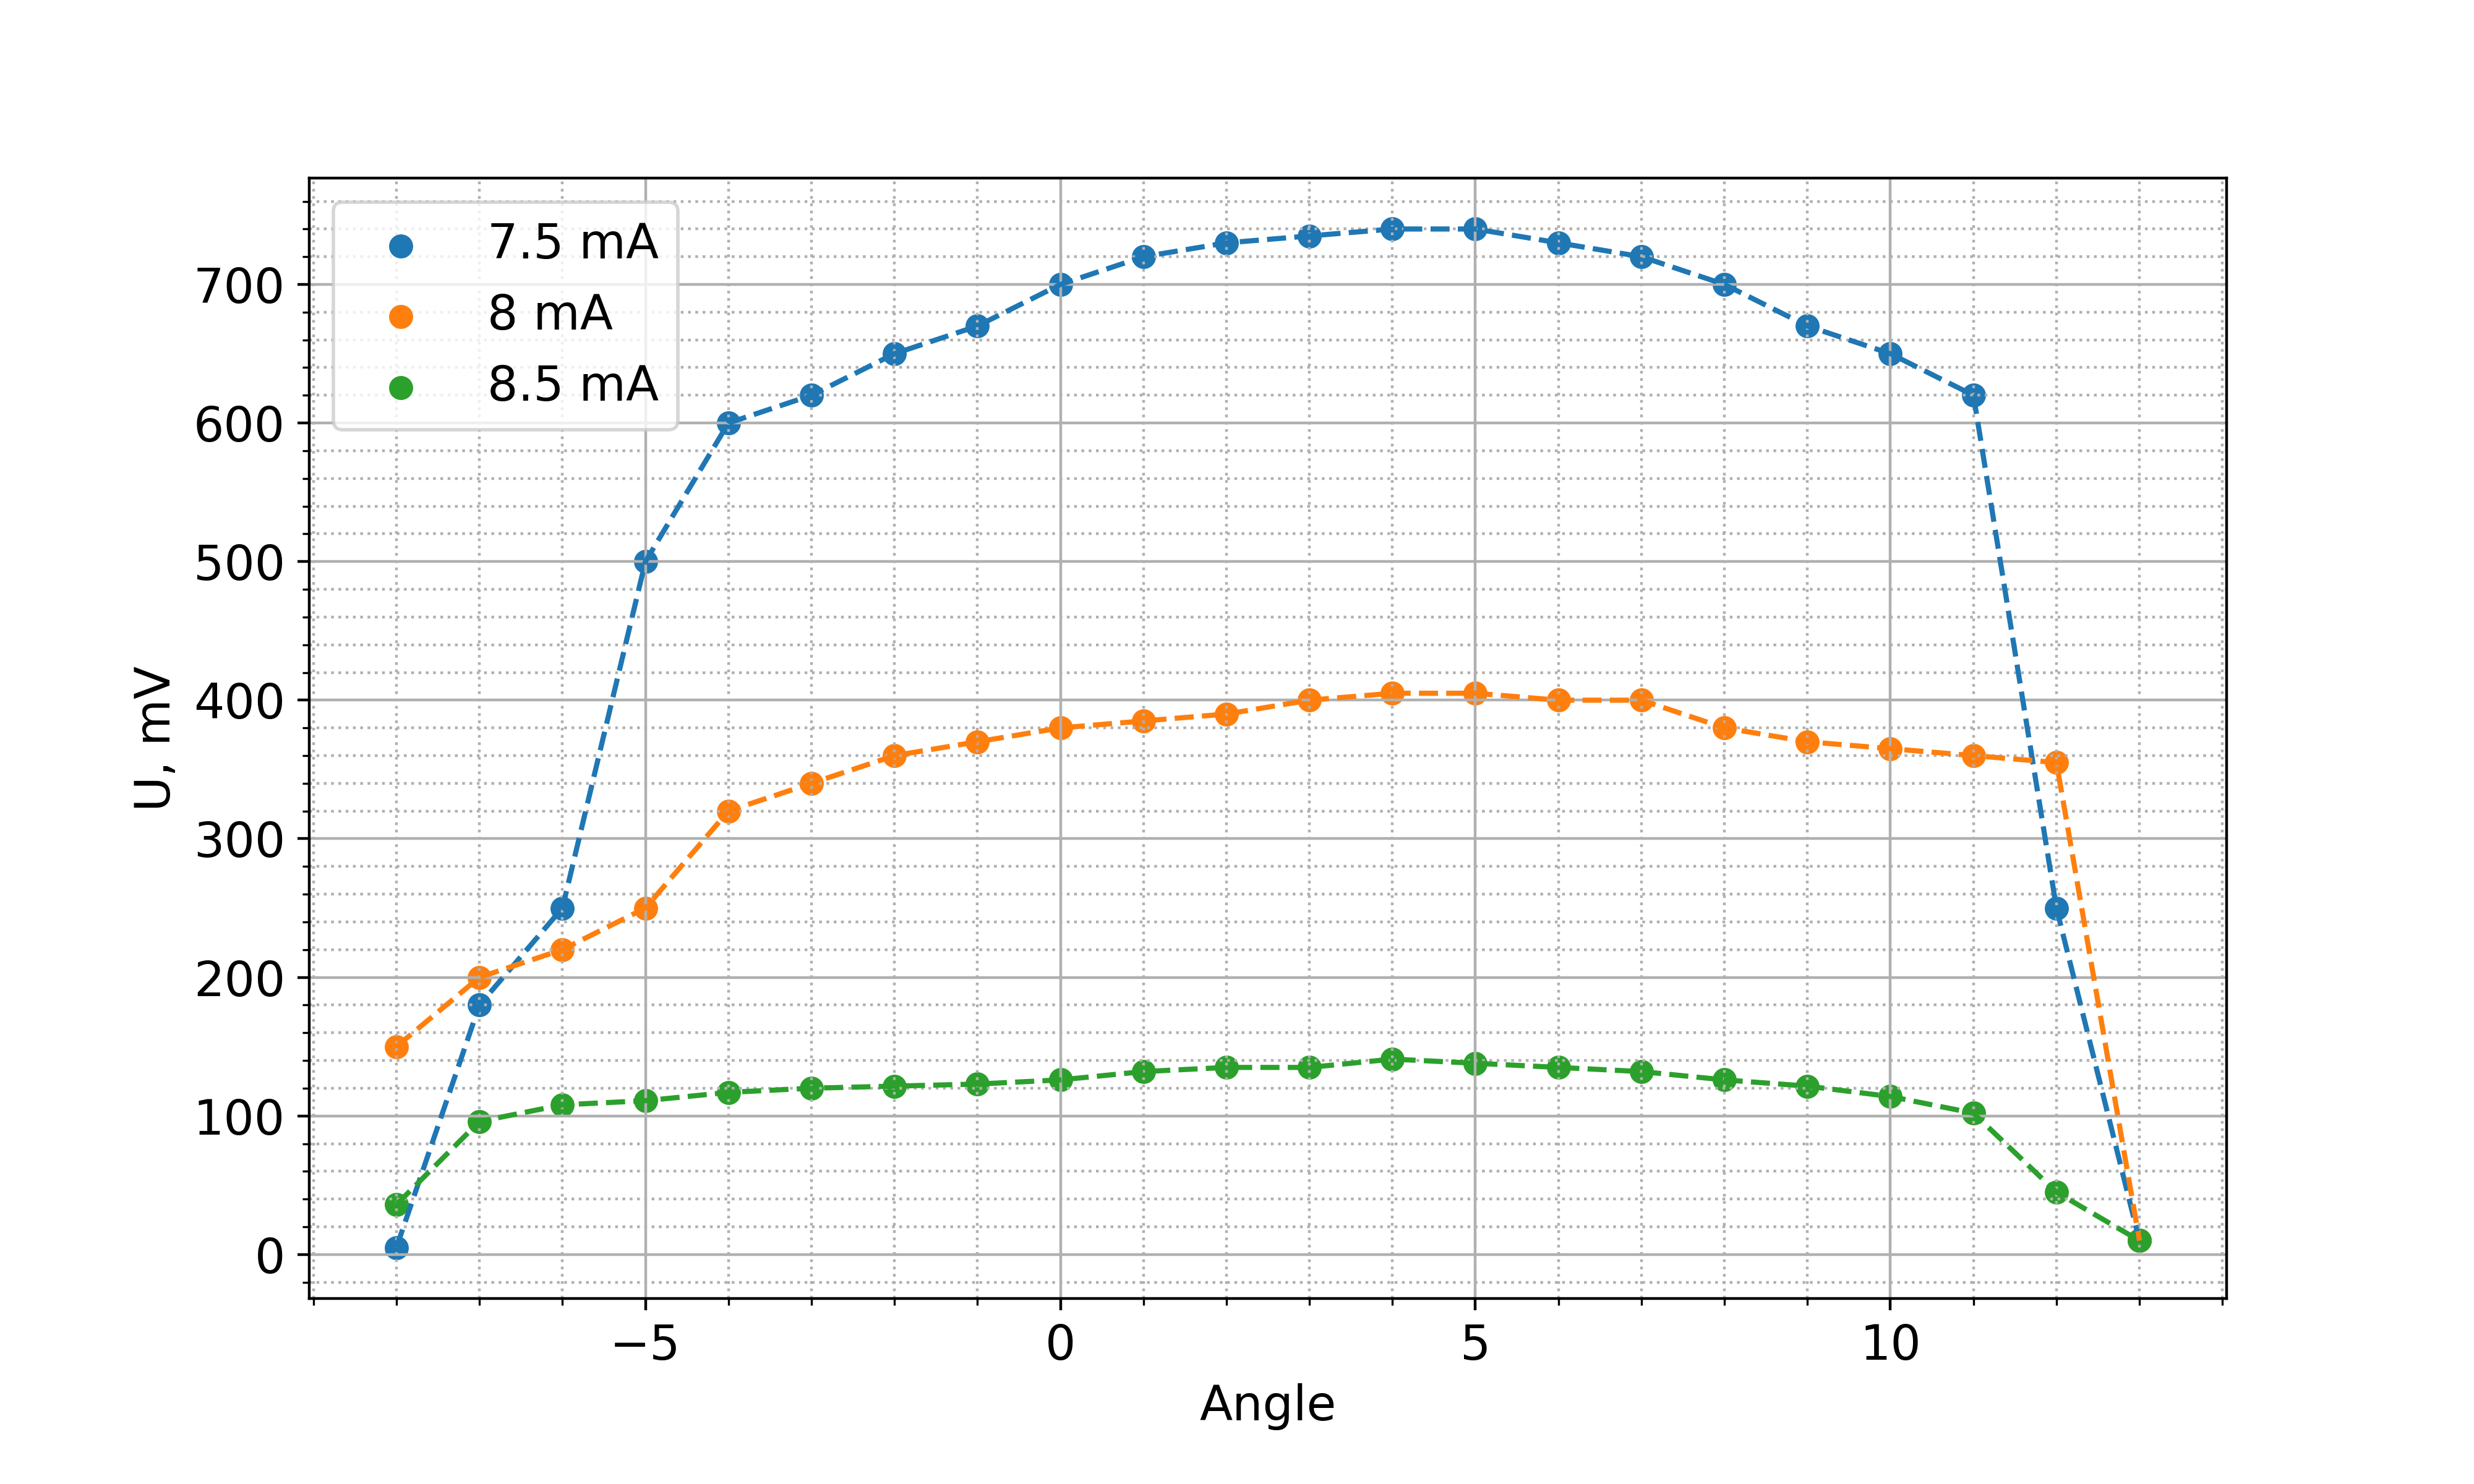
\includegraphics[scale=0.5]{g1.png}
        \caption{U(Angle)}
        \label{g1}
    \end{center}
\end{figure}


\subsection{Щель расположена параллельно активному слою}

\begin{figure}[H]
    \begin{center}
        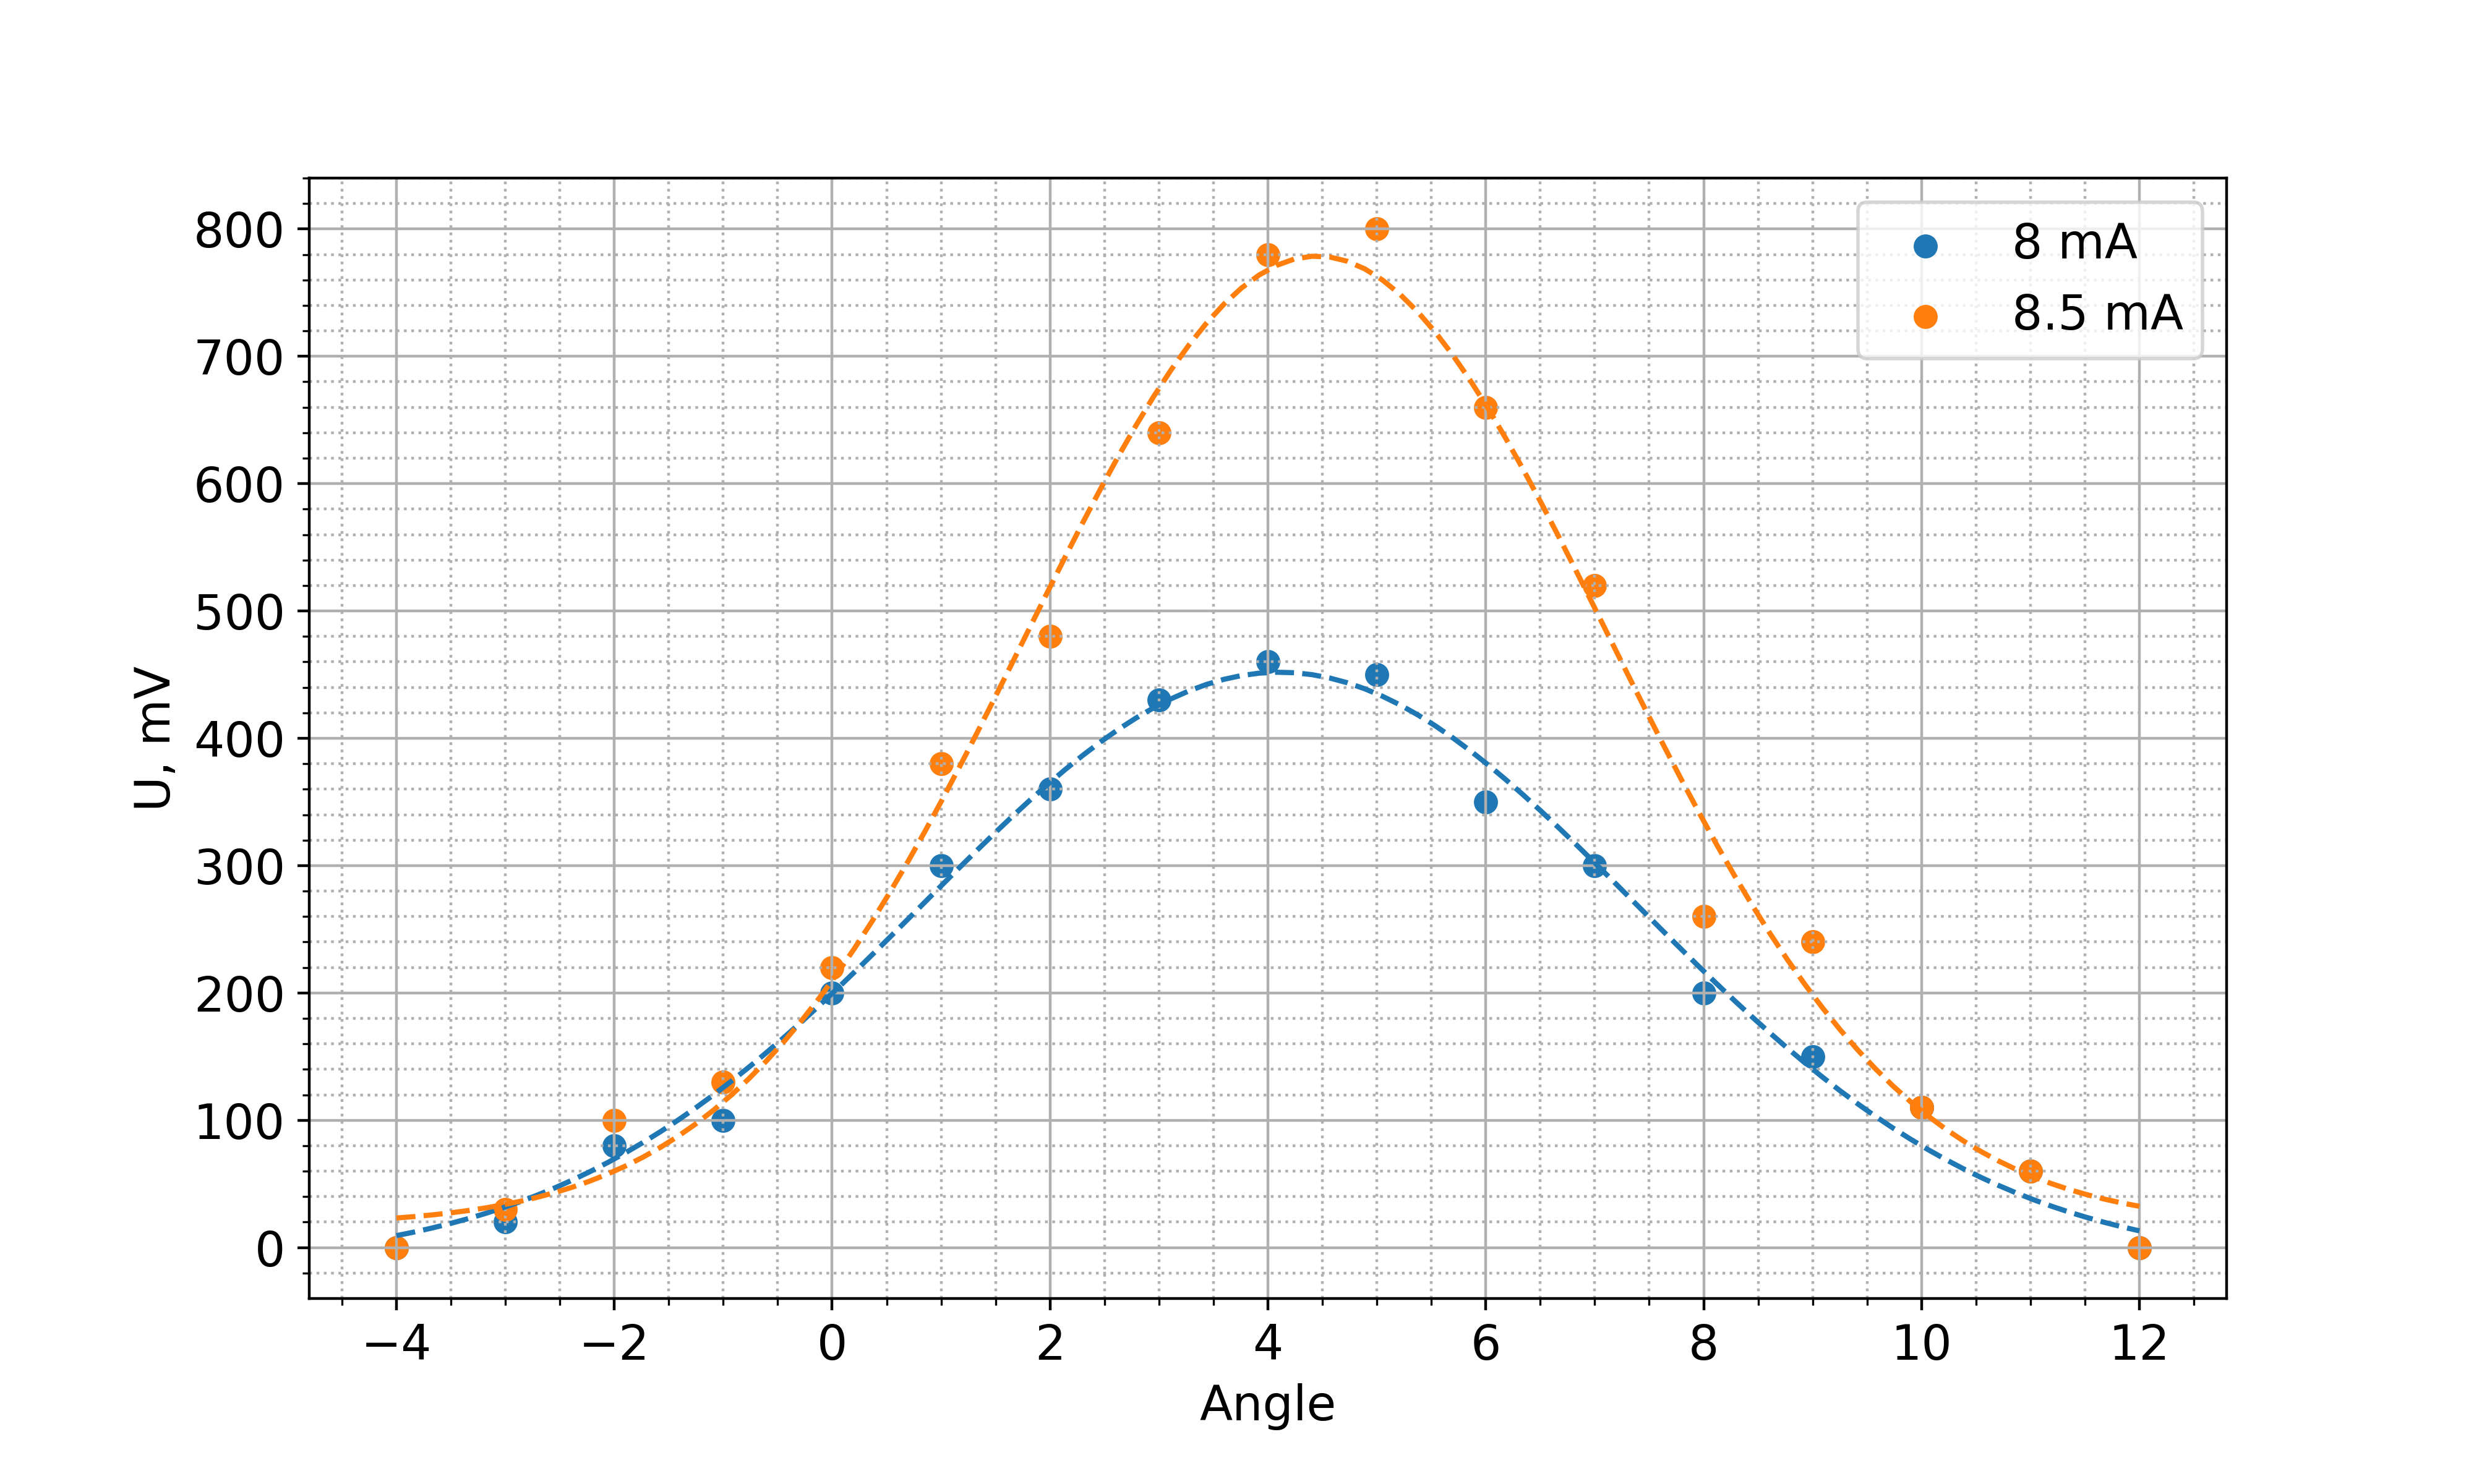
\includegraphics[scale=0.5]{g2.png}
        \caption{U2(Angle)}
        \label{g2}
    \end{center}
\end{figure}

\begin{table}[h]
\centering
\caption{Коэффициенты аппроксимации $I=8\; mA$}
\label{coeffs_table}
\begin{tabular}{lrr}
\toprule
coeffs &  coef\_values &  standart\_error \\
\midrule
    U0 &   -12.549157 &       16.503157 \\
     A &     4.106410 &        0.076892 \\
    xc &    -6.560648 &        0.327160 \\
     w & -3818.948496 &      285.046729 \\
\bottomrule
\end{tabular}
\end{table}

\begin{table}[h]
\centering
\caption{Коэффициенты аппроксимации $I=8.5\; mA$}
\label{coeffs_table}
\begin{tabular}{lrr}
\toprule
coeffs &  coef\_values &  standart\_error \\
\midrule
    U0 &    17.921781 &       20.133823 \\
     A &     4.451687 &        0.081142 \\
    xc &     5.363032 &        0.252814 \\
     w &  5113.828306 &      313.554494 \\
\bottomrule
\end{tabular}
\end{table}



\par Делали фит гауссовского пучка:
	
	    \begin{equation}
	        U = U_0 + \frac{A}{w \sqrt{\pi / 2}} e^{-2 \frac{(\alpha - \alpha_0)^2}{w^2}}
	    \end{equation}
	
	Получим толщину активной зоны:
	
	    \begin{equation}
	        d = \frac{1}{2} \frac{\lambda}{\sigma} = \frac{1}{4} (\frac{652}{2.68} + \frac{652}{3.28}) = 111 \: \hbox{нм} \approx \frac{1}{6} \lambda
	    \end{equation}


\newpage
\section{Выводы}


    \begin{itemize}
        \item Провели измерения напряжения на фотодетекторе от угла его поворота относительно направления излучения лазера в плоскости активного слоя и плоскости, перпендикулярной активному слою;
        \item При параллельном расположении щели и активного слоя измерения хорошо аппроксимируются гауссианами с ошибками порядка единиц процентов;
        \item Оценилили толщину активного слоя $\sim \frac{\lambda}{6}$;
        \item Зависимость $U(\alpha)$ при взаимноперпендикулярного расположении щели и активного слоя не соответсвует гауссовому, что говорит нам об искажениях сигнала ввиду внесения ограничений в его распространени с помощью щели;
    \end{itemize}


\end{document}